\documentclass[a4paper, oneside]{memoir}
\usepackage[utf8]{inputenc}
\usepackage[T1]{fontenc}
\usepackage{pifont}
\usepackage{amssymb}
\usepackage{fourier}
\usepackage[dvipsnames]{xcolor}
\usepackage{tikz}
\usepackage{pdfpages}
\usepackage[sfdefault]{roboto}
\usepackage{color}

% Styles
\tikzstyle{teamshare} = [below, text width=5.4cm, inner sep = 0.5cm, text=white, align=center]
\tikzstyle{cardtext} = [below, text width=5.9cm, inner sep = 0.25cm, text centered]
\setlrmarginsandblock{0.9cm}{*}{1}
\setulmarginsandblock{1.2cm}{*}{1}
\checkandfixthelayout[nearest]
\pagestyle{empty}

% Define Commands
\newcommand{\condition}[1]{\textbf{#1}}
\newcommand{\character}[1]{\textbf{#1}}
\newdimen\titlespacing
\titlespacing=0.15cm

% Define Seperators
\newcommand{\seperator}[1]{\\ \vspace{\titlespacing} \hrulefill {} \tiny \bfseries #1 \normalfont \normalsize \hrulefill \\ \vspace{\titlespacing}}
\newcommand{\seperatoraction}{\seperator{POWER}}
\newcommand{\seperatordescription}{\seperator{DESCRIPTION}}
\newcommand{\seperatorcondition}{\seperator{CONDITION}}
\newcommand{\seperatorwin}{\seperator{HOW TO WIN}}
\newcommand{\redwinsection}{
	\seperatorwin
	You win if \character{Harry Potter} avoids \\ the \condition{Avada Kadavra} curse.
}
\newcommand{\greenwinsection}{
	\seperatorwin
	\small You win if \character{Harry Potter} gets hit by the \condition{Avada Kadavra} curse.
}
\newcommand{\titlefrom}[1]{\\ \tiny > from #1 <\normalsize}

% Begin Document
\begin{document}
	
% New Page
\noindent 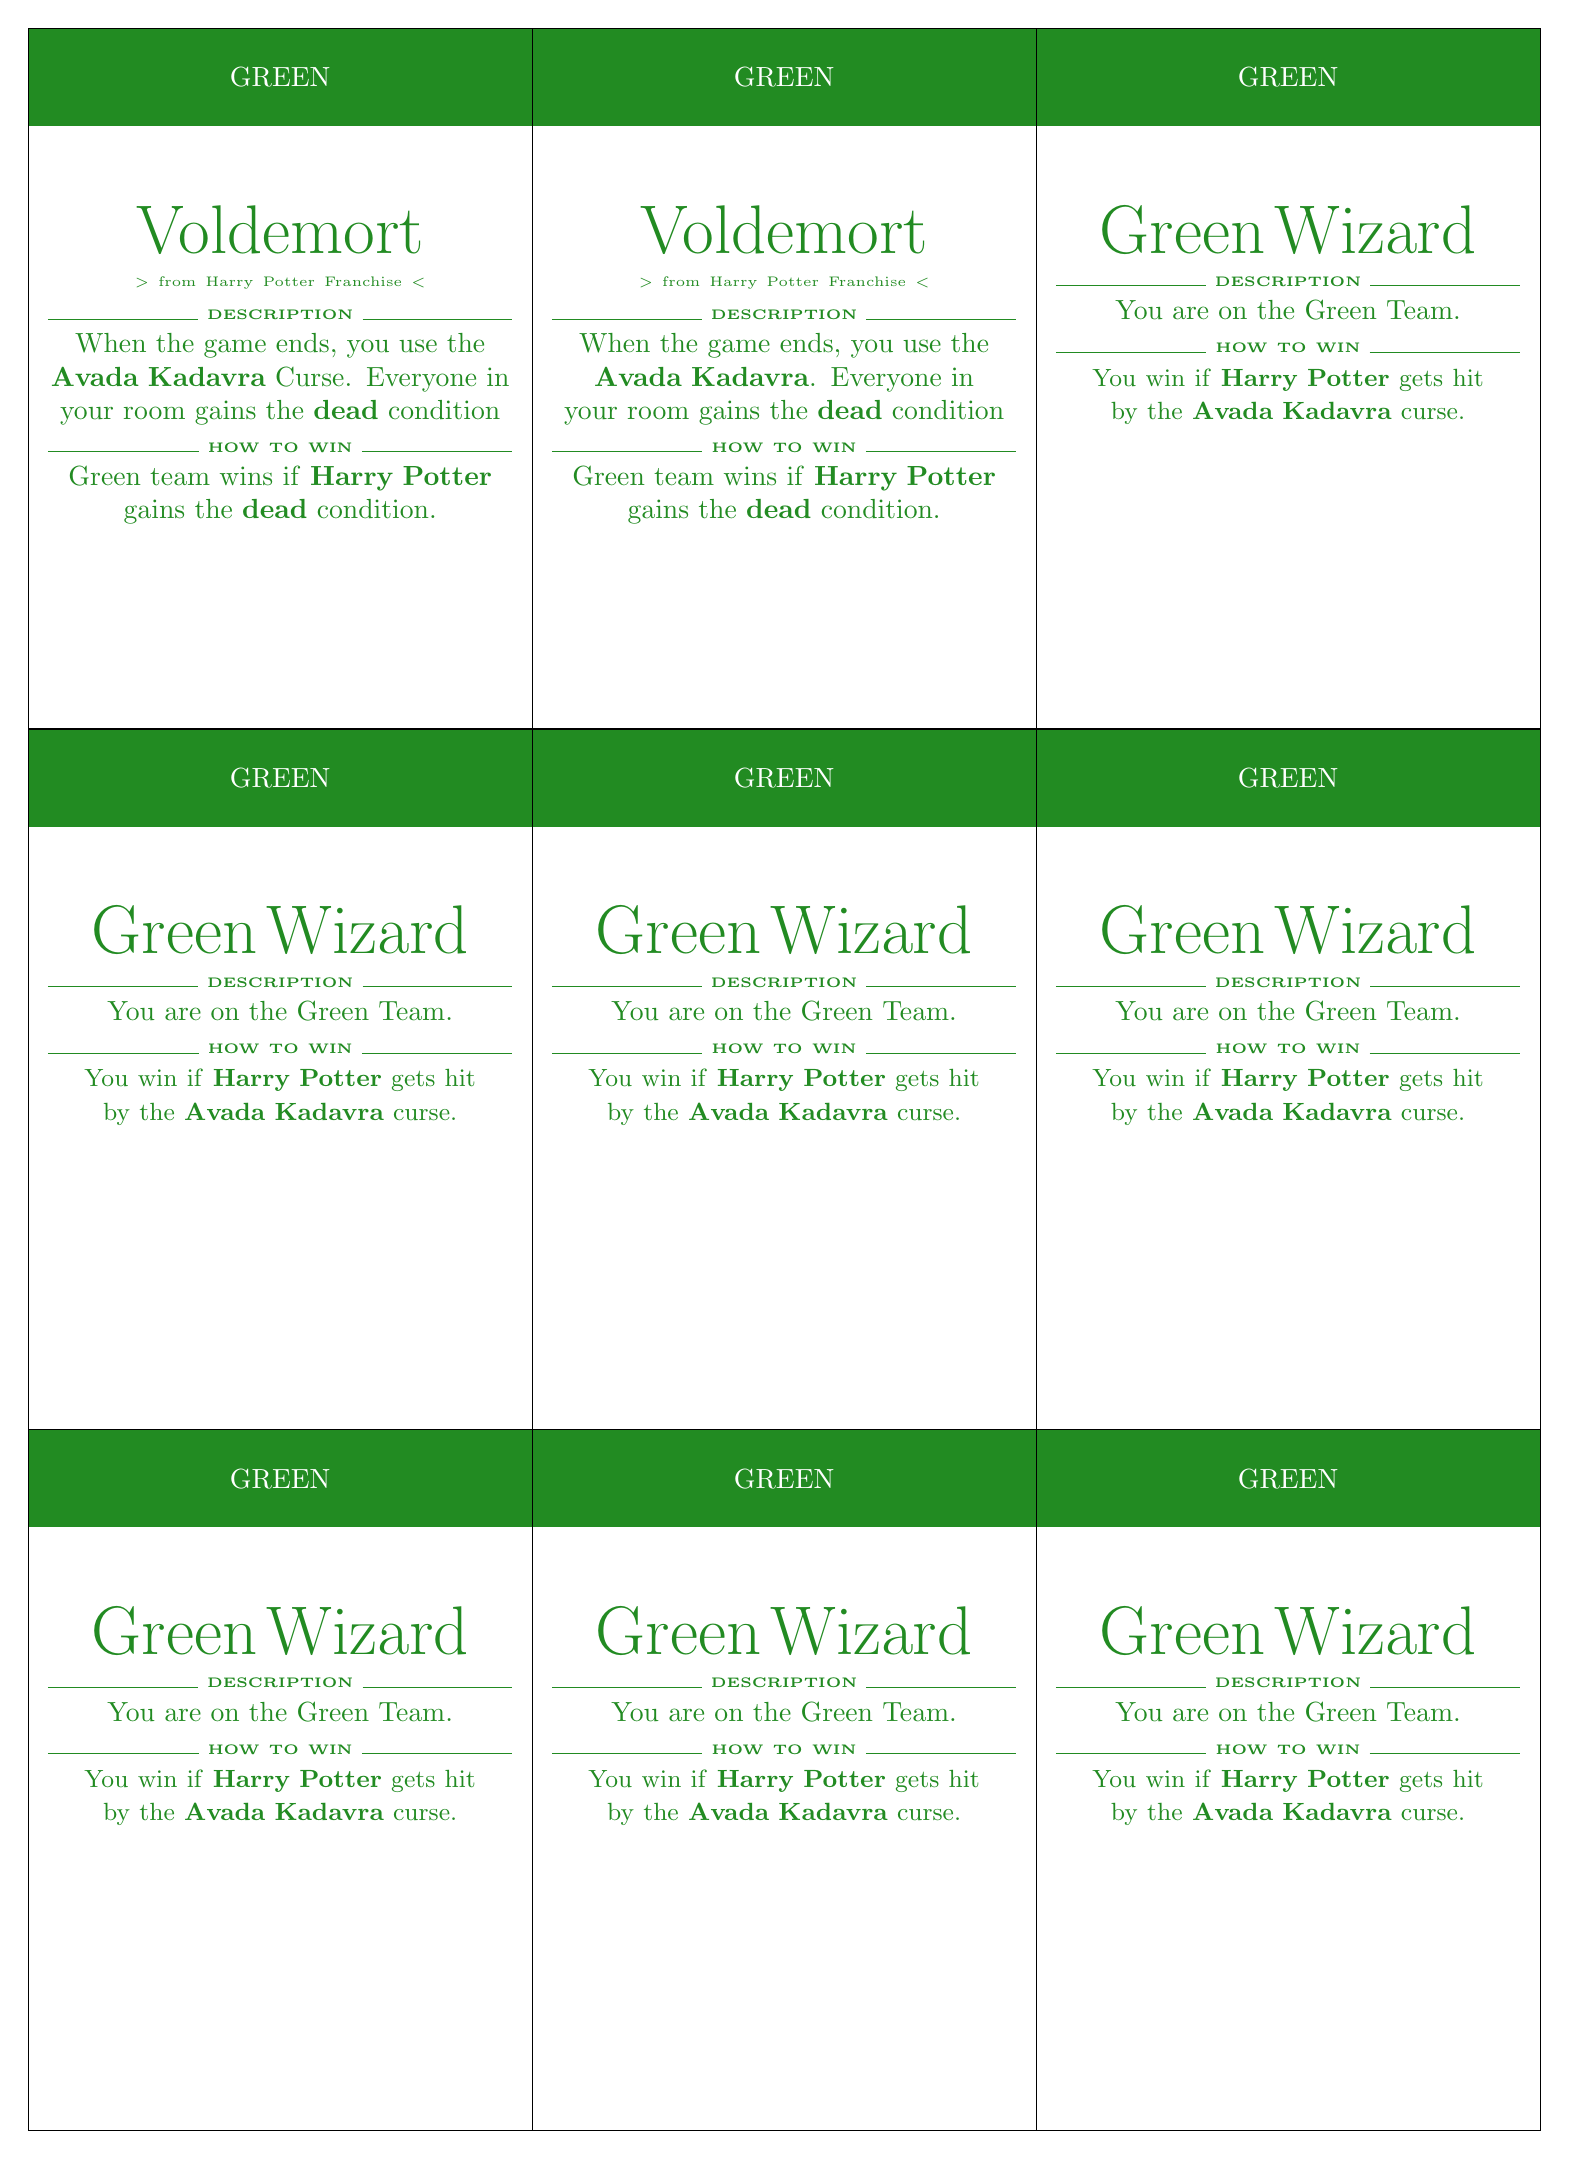
\begin{tikzpicture}[outer sep=0]

	% VOLDEMORT
	\node[teamshare, fill=ForestGreen] (1) at (3.2,26.7) {\HUGE GREEN};
	\node[cardtext, text=ForestGreen] at (3.2,24.7) {
		{\Huge Voldemort}
		\titlefrom{Harry Potter Franchise}
		\seperatordescription
		When the game ends, you use the \condition{Avada Kadavra} Curse. Everyone in your room gains the \condition{dead} condition
		\seperatorwin
		Green team wins if \character{Harry Potter} \\ gains the \condition{dead} condition.
	};
	
	% VOLDEMORT
	\node[teamshare, fill=ForestGreen] at (9.6,26.7) {\HUGE GREEN};
	\node[cardtext, text=ForestGreen] at (9.6,24.7) {
		{\Huge Voldemort}
		\titlefrom{Harry Potter Franchise}
		\seperatordescription
		When the game ends, you use the \condition{Avada Kadavra}. Everyone in your room gains the \condition{dead} condition
		\seperatorwin
		Green team wins if \character{Harry Potter} \\ gains the \condition{dead} condition.
	};
	
	% GREEN WIZARD
	\node[teamshare, fill=ForestGreen] at (16,26.7) {\HUGE GREEN};
	\node[cardtext, text=ForestGreen] at (16,24.7) {
		{\Huge Green Wizard}
		\seperatordescription
		You are on the Green Team.
		\greenwinsection
	};
	
	% GREEN WIZARD
	\node[teamshare, fill=ForestGreen] at (3.2,17.8) {\HUGE GREEN};
	\node[cardtext, text=ForestGreen] at (3.2,15.8) {
		{\Huge Green Wizard}
		\seperatordescription
		You are on the Green Team.
		\greenwinsection
	};
	
	% GREEN WIZARD
	\node[teamshare, fill=ForestGreen] at (9.6,17.8) {\HUGE GREEN};
	\node[cardtext, text=ForestGreen] at (9.6,15.8) {
		{\Huge Green Wizard}
		\seperatordescription
		You are on the Green Team.
		\greenwinsection
	};
	
	% GREEN WIZARD
	\node[teamshare, fill=ForestGreen] at (16,17.8) {\HUGE GREEN};
	\node[cardtext, text=ForestGreen] at (16,15.8) {
		{\Huge Green Wizard}
		\seperatordescription
		You are on the Green Team.
		\greenwinsection
	};
	
	% GREEN WIZARD
	\node[teamshare, fill=ForestGreen] at (3.2,8.9) {\HUGE GREEN};
	\node[cardtext, text=ForestGreen] at (3.2,6.9) {
		{\Huge Green Wizard}
		\seperatordescription
		You are on the Green Team.
		\greenwinsection
	};
	
	% GREEN WIZARD
	\node[teamshare, fill=ForestGreen] at (9.6,8.9) {\HUGE GREEN};
	\node[cardtext, text=ForestGreen] at (9.6,6.9) {
		{\Huge Green Wizard}
		\seperatordescription
		You are on the Green Team.
		\greenwinsection
	};
	
	% GREEN WIZARD
	\node[teamshare, fill=ForestGreen] at (16,8.9) {\HUGE GREEN};
	\node[cardtext, text=ForestGreen] at (16,6.9) {
		{\Huge Green Wizard}
		\seperatordescription
		You are on the Green Team.
		\greenwinsection
	};
	
	\draw (0,0) -- (19.2,0);
	\draw (0,8.9) -- (19.2,8.9);
	\draw (0,17.8) -- (19.2,17.8);
	\draw (0,26.7) -- (19.2,26.7);
	
	\draw (0,0) -- (0,26.7);
	\draw (6.4,0) -- (6.4,26.7);
	\draw (12.8,0) -- (12.8,26.7);
	\draw (19.2,0) -- (19.2,26.7);



\end{tikzpicture}

%Background is not my own. But courtesy of a user on BGG

\includepdf[pages={1}, angle=0]{cardsbackground.pdf}
\pagebreak

\noindent 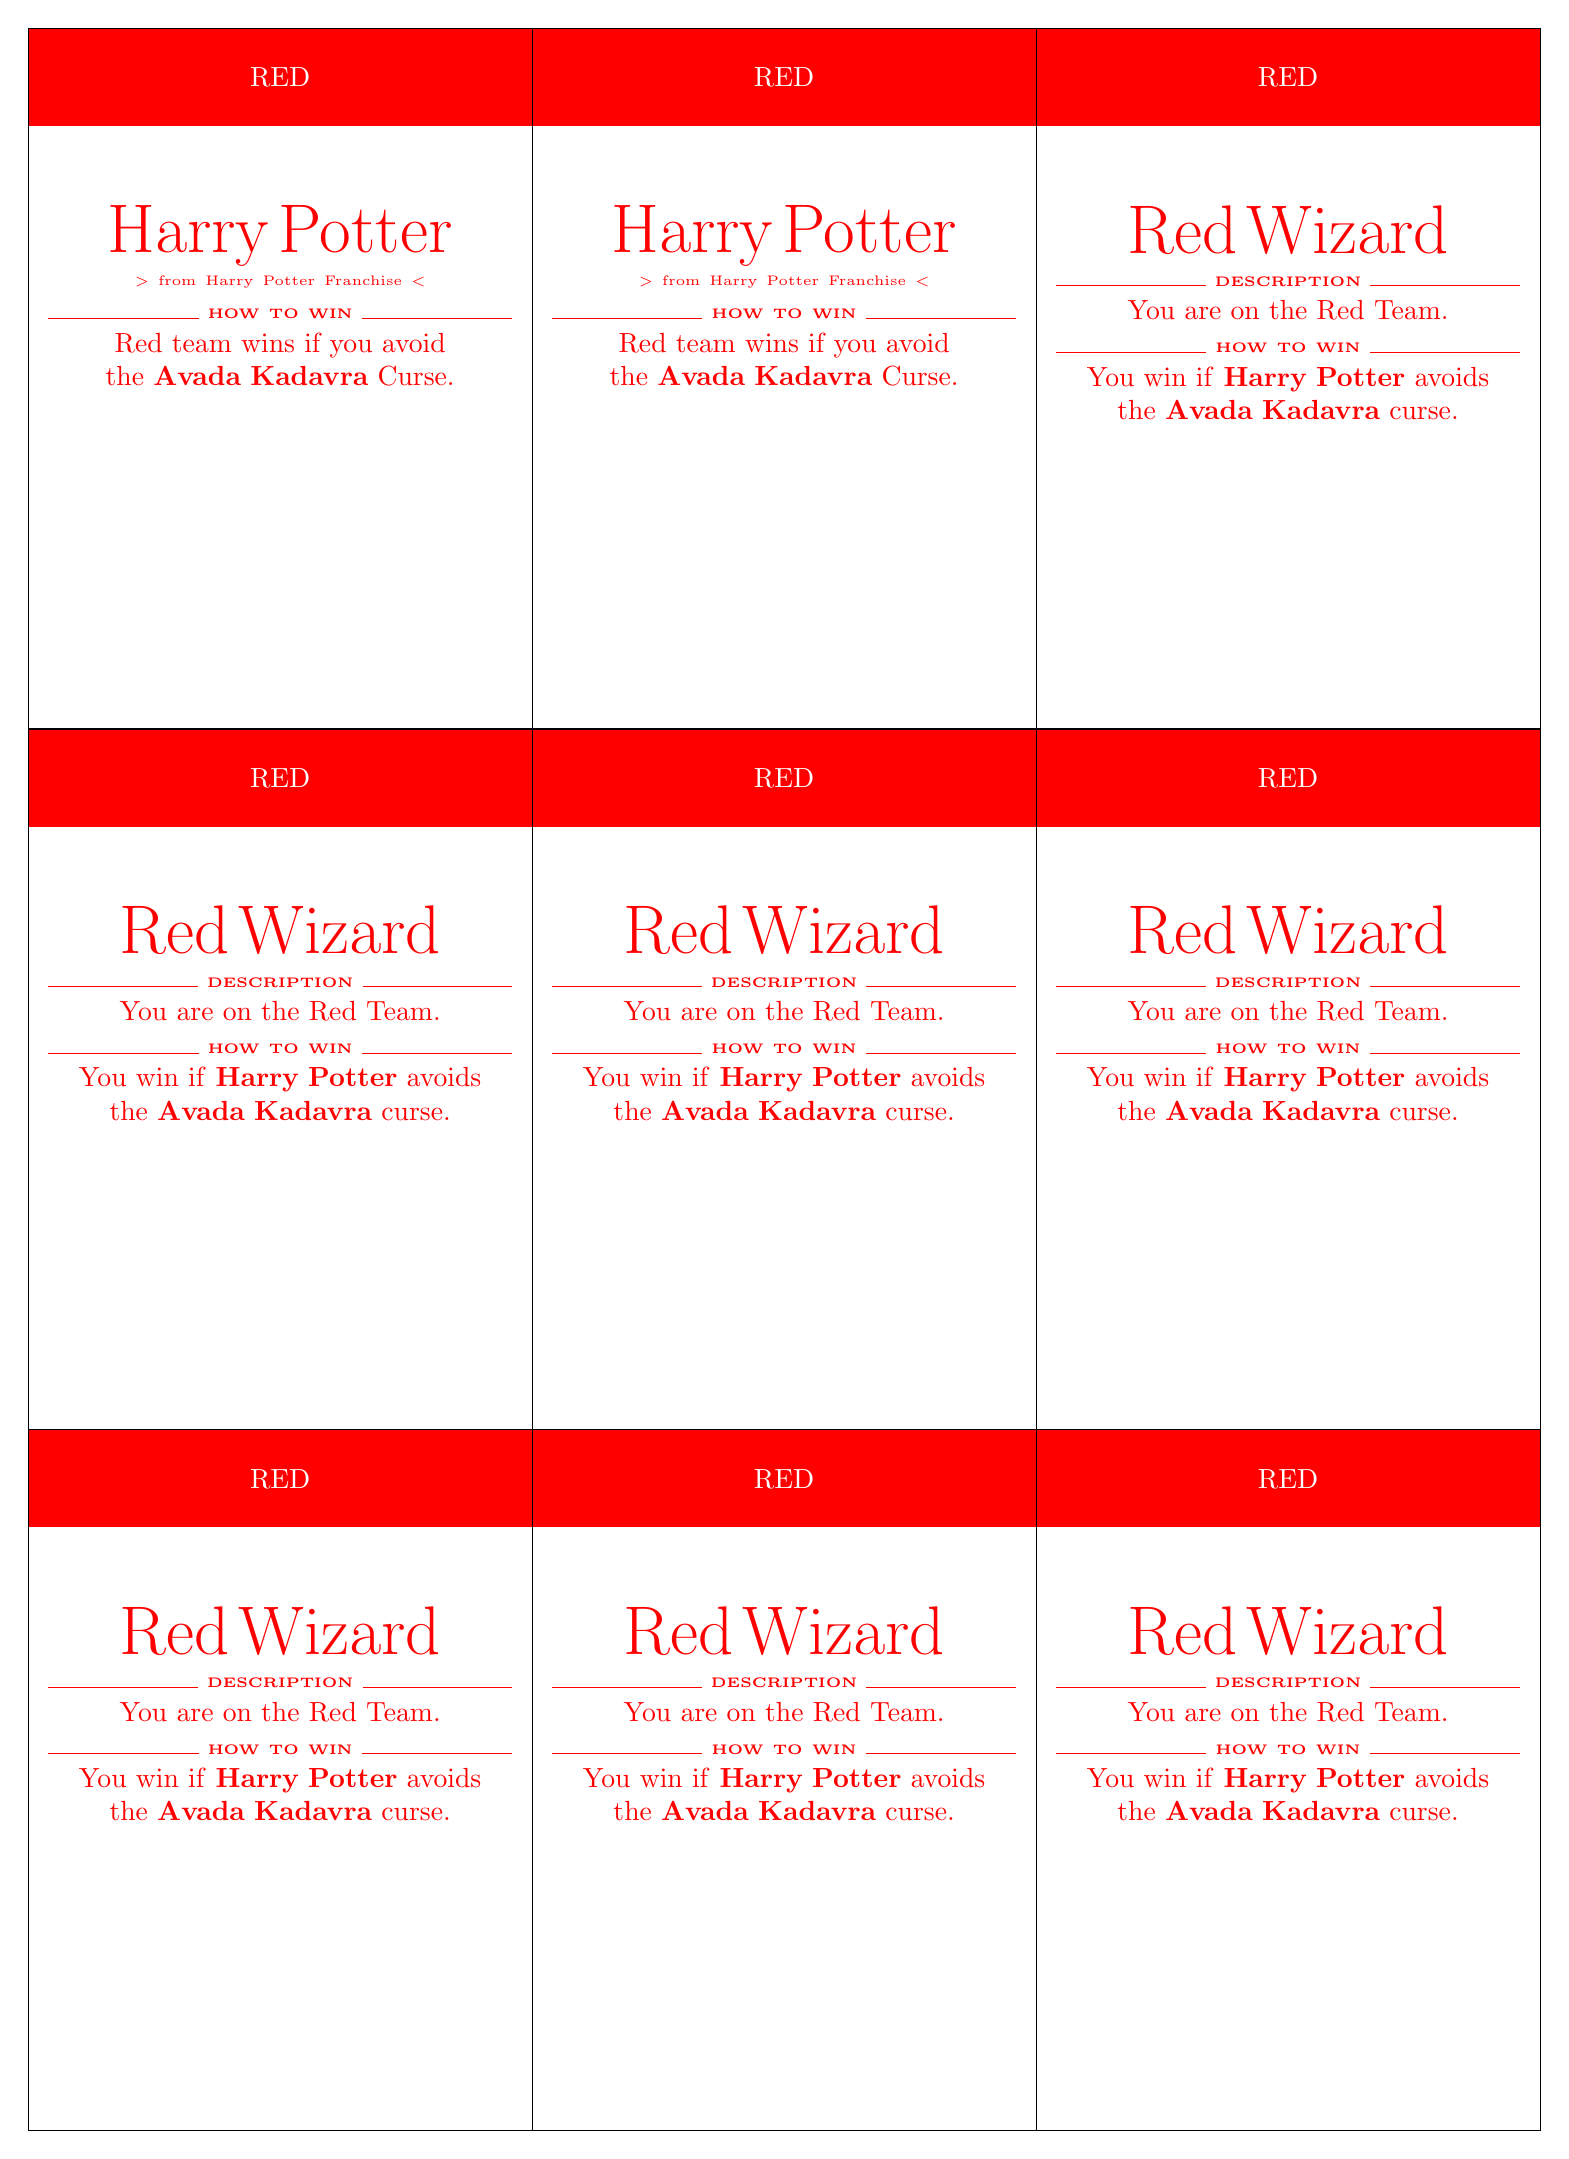
\begin{tikzpicture}[outer sep=0]

	% HARRY POTTER
	\node[teamshare, fill=red] (1) at (3.2,26.7) {\HUGE RED};
	\node[cardtext, text=red] at (3.2,24.7) {
		{\Huge Harry Potter}
		\titlefrom{Harry Potter Franchise}
		\seperatorwin
		Red team wins if you avoid the \condition{Avada Kadavra} Curse.
	};
	
	% HARRY POTTER
	\node[teamshare, fill=red] at (9.6,26.7) {\HUGE RED};
	\node[cardtext, text=red] at (9.6,24.7) {
		{\Huge Harry Potter}
		\titlefrom{Harry Potter Franchise}
		\seperatorwin
		Red team wins if you avoid the \condition{Avada Kadavra} Curse.
	};
	
	% RED WIZARD
	\node[teamshare, fill=red] at (16,26.7) {\HUGE RED};
	\node[cardtext, text=red] at (16,24.7) {
		{\Huge Red Wizard}
		\seperatordescription
		You are on the Red Team.
		\redwinsection
	};
	
	% RED WIZARD
	\node[teamshare, fill=red] at (3.2,17.8) {\HUGE RED};
	\node[cardtext, text=red] at (3.2,15.8) {
		{\Huge Red Wizard}
		\seperatordescription
		You are on the Red Team.
		\redwinsection
	};
	
	% RED WIZARD
	\node[teamshare, fill=red] at (9.6,17.8) {\HUGE RED};
	\node[cardtext, text=red] at (9.6,15.8) {
		{\Huge Red Wizard}
		\seperatordescription
		You are on the Red Team.
		\redwinsection
	};
	
	% RED WIZARD
	\node[teamshare, fill=red] at (16,17.8) {\HUGE RED};
	\node[cardtext, text=red] at (16,15.8) {
		{\Huge Red Wizard}
		\seperatordescription
		You are on the Red Team.
		\redwinsection
	};
	
	% RED WIZARD
	\node[teamshare, fill=red] at (3.2,8.9) {\HUGE RED};
	\node[cardtext, text=red] at (3.2,6.9) {
		{\Huge Red Wizard}
		\seperatordescription
		You are on the Red Team.
		\redwinsection
	};
	
	% RED WIZARD
	\node[teamshare, fill=red] at (9.6,8.9) {\HUGE RED};
	\node[cardtext, text=red] at (9.6,6.9) {
		{\Huge Red Wizard}
		\seperatordescription
		You are on the Red Team.
		\redwinsection
	};
	
	% RED WIZARD
	\node[teamshare, fill=red] at (16,8.9) {\HUGE RED};
	\node[cardtext, text=red] at (16,6.9) {
		{\Huge Red Wizard}
		\seperatordescription
		You are on the Red Team.
		\redwinsection
	};
	
	\draw (0,0) -- (19.2,0);
	\draw (0,8.9) -- (19.2,8.9);
	\draw (0,17.8) -- (19.2,17.8);
	\draw (0,26.7) -- (19.2,26.7);
	\draw (0,0) -- (0,26.7);
	\draw (6.4,0) -- (6.4,26.7);
	\draw (12.8,0) -- (12.8,26.7);
	\draw (19.2,0) -- (19.2,26.7);

\end{tikzpicture}

\includepdf[pages={1}, angle=0]{cardsbackground.pdf}

\end{document}